\Echapter{Quantifying Arterial Spin Labeling Data}{Swati D. Rane}{srleven@uw.edu}

This is an example
of how to use a makefile to quantify cerebral blood flow (CBF) from
pseudo-continuous arterial spin labeling (pCASL) data. 

The code for this example is in
\texttt{\$MAKEPIPELINES/ASLTestsubject/S001/Makefile}. S001 is the
name of the subject and the folder name. In this example 
we assume we have one folder per subject. The folder name
reflects the subject name and contains the
\texttt{SUBJECTNAME_ASL.nii.gz} and \texttt{SUBJECTNAME_M0.nii.gz}
files. The ASL file contains alternating volumes from the control and
label acquisitions, where the odd volumes are control volumes and the even
volumes are the label volumes. The M0 file is a single 3D volume of
the reference proton density weighted image.

A unique feature of this example is that we have
performed surround subtraction in MATLAB to improve the 
signal-to-noise ratio of the ASL data.  We have included a standalone 
MATLAB application that can be installed with the necessary runtime binaries 
and libraries to complete this step. Note that this approach does not  
require you to have MATLAB installed on your computer. Similarly, if
you have a limited number of floating licenses available, deploying a
standalone MATLAB application does not require a floating license. 

If you are not at IBIC, before running this example you must install
the MATLAB runtime libraries and surround subtraction application as follows:
\\
Change directory to \texttt{ASLTestsubject/bin} and run the program
\texttt{SSInstaller_mcr.install} as shown in \autoref{bash:matlab}.
\begin{bash}{Installing MATLAB Runtime Libraries and surround
    subtraction application}{bash:matlab}
cd \$MAKEPIPELINES/ASLTestsubject/S001/Makefile\\
./SSInstaller_mcr.install
\end{bash}

\begin{figure}
\begin{center}
  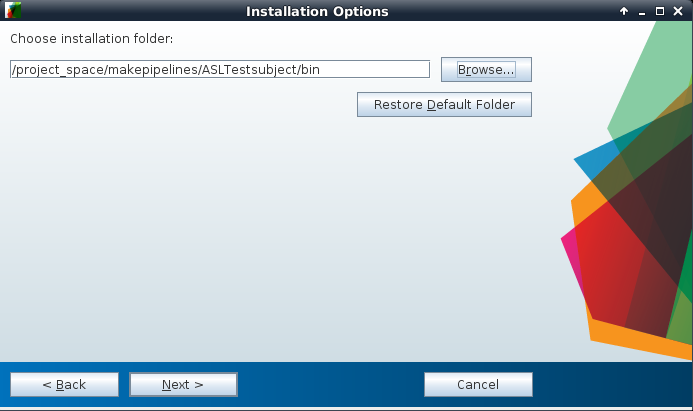
\includegraphics[scale=.6]{images/installApp2.png}
\caption{Entering location of installation folder for Surround 
  Subtraction standalone MATLAB application.}
\label{fig:ssinstall2}
\end{center}
\end{figure}

The installer will, perhaps after some delay, open a splash screen
with an opportunity to change connection settings. Just click next.
The next screens will prompt for a location for the installation folder
(see \autoref{fig:ssinstall2}). Enter the location of
\texttt{\$MAKEPIPELINES/ASLTestsubject/bin} whenever asked. Note that
here, the value of \texttt{MAKEPIPELINES} is set to
\texttt{/project_space/makepipelines}. In your environment this will
be different.
\clearpage

\begin{lstlisting}
	SHELL=/bin/bash

	%*\lnote*tau = 1.5
	pld = 1.525
	label_eff = 0.85
	T1b = 1.627
	lambda=0.9

	ifeq "$(origin MAKEPIPELINES)" "undefined"
	MAKEPIPELINES=/project_space/makepipelines
	endif

	PROJECT_HOME = $(MAKEPIPELINES)/ASLTestsubject/S001

	%*\lnote*#FSLDIR=/usr/share/fsl/5.0
	FSL_PATH = ${FSLDIR}/bin


	%*\lnote*MATLAB_PATH = $(MAKEPIPELINES)/ASLTestsubject/bin
	STD_BRAIN2mm = ${FSLDIR}/data/standard/MNI152_T1_2mm_brain.nii.gz
	STD_BRAIN2mm_MASK = ${FSLDIR}/data/standard/MNI152_T1_2mm_brain_mask.nii.gz
	STD_BRAIN2mm_GM = ${FSLDIR}/data/standard/tissuepriors/avg152T1_gray.img

	SUBJECT = $(shell basename ${PROJECT_HOME})	
\end{lstlisting}

\lnum{1}CBF quantification requires specific sequence parameters such as label duration (\texttt{tau}), post labeling delay (\texttt{pld}), longitudinal relaxation, T1 of blood (\texttt{T1b}). \texttt{label_eff} and \texttt{lambda} are constants defining the labeling efficiency for pCASL and the tissue-blood partition coefficient respectively. For convenience, we have predefined the paths for subject directory \texttt{PROJECT_HOME} as well as standard template brains and masks under \texttt{STD_BRAIN2mm}, \texttt{STD_BRAIN2mm_MASK}, and \texttt{STD_BRAIN2mm_GM}. 

\lnum{2}Because we have multiple versions of FSL installed, we set variables to describe what version of FSL we are using in the Makefile. 

\lnum{3} The MALTAB app is a \texttt{.mcr} file. Double clicking will open an installation window to copy the codes to a user-specified location. In this project, we have copied these files and folders in the \texttt{bin} directory under \texttt{ASLTestSubject}. This can serve as the common directory for all subjects. The \texttt{surround_subtraction.sh} is the shell file that calls \texttt{run_Surround_Subtraction.sh} generated by the MATLAB app. 
 
\begin{lstlisting}
	.PHONY =  all clean
	all:${SUBJECT}_CBF_MNI.nii.gz  QA/ASL.gif
	
	${SUBJECT}_mc_ASL.nii.gz: ${SUBJECT}_ASL.nii.gz ${SUBJECT}_M0.nii.gz
		${FSL_PATH}/mcflirt -in $< -reffile $(word 2,$^) -out $@;
\end{lstlisting}

In this segment of code, we motion correct the ASL data using MCFLIRT in FSL. Because the ASL and M0 data are acquired as separate scans, all ASL volumes are registered to the M0 volume. This is unlike the motion correction typically performed in BOLD fMRI where the central dynamic is considered as the reference volume. All remaining volumes are registered to this central volume.

\begin{lstlisting}
	#Implement surround subtraction for calculating differences in MATLAB
	%*\lnote*${SUBJECT}_DeltaM.nii.gz: ${SUBJECT}_mc_ASL.nii.gz 
		${MATLAB_PATH}/surround_subtraction.sh $< ${MATLAB_PATH} 
	
	%*\lnote*${SUBJECT}_CBF.nii.gz:${SUBJECT}_DeltaM.nii.gz ${SUBJECT}_M0.nii.gz;
		${FSL_PATH}/fslmaths $< -div $(word 2,$^) temp;\
		${FSL_PATH}/fslmaths temp -mul $(shell echo "scale=5; 6000*${lambda};" | bc -l) temp ;\
		${FSL_PATH}/fslmaths temp -mul  $(shell echo "scale=5; e(${pld}/${T1b});" | bc -l) temp;\
		${FSL_PATH}/fslmaths temp -div $(shell echo "scale=5; 2*${label_eff}*${T1b}*(1-e(-${tau}/${T1b}));" | bc -l) $@;\
		rm temp.nii.gz
\end{lstlisting}

In this section, we compute absolute values of CBF. \lnum{4} The \texttt{surround_subtraction.sh} script evaluates the dimensions of the ASL data (rows, columns, slices) and calls the MATLAB script via \texttt{run_Surround_Subtraction.sh}. \lnum{5} CBF is computed in ml/100gm/min, using ASL white paper MRM 73:102 (2015). 

\begin{lstlisting}
	${SUBJECT}_CBF_MNI.nii.gz: ${SUBJECT}_M0.nii.gz ${SUBJECT}_CBF.nii.gz
		${FSL_PATH}/flirt -in $< -ref ${STD_BRAIN2mm} -out temp.nii.gz -omat cbf_to_MNI.mat -bins 256 -cost corratio -searchrx -90 90 -searchry -90 90 -searchrz -90 90 -dof 12  -interp trilinear;\
		${FSL_PATH}/flirt -in $(word 2, $^) -ref ${STD_BRAIN2mm} -out temp.nii.gz -applyxfm -init cbf_to_MNI.mat;\
		${FSL_PATH}/fslmaths temp.nii.gz -mul ${STD_BRAIN2mm_MASK} $@;\
		rm temp.nii.gz
\end{lstlisting}

This portion of the Makefile registers the CBF map to MNI space and
removes background. We did not have a corresponding T1 image for this
ASL data. Hence we regististered the M0 image directly to the the
standard 2mm MNI template available in FSL. We then applied the
subsequent transformation matrix to the CBF map. 

Ideally, if a T1 image were available, this step would be
different. We would register the M0 image to the subject's native T1
image. The T1 image would be registered to the MNI template, and we
would combine the two transformation matrices to register the CBF map
to MNI space.

\begin{lstlisting}
	QA/ASL.png:${SUBJECT}_CBF_MNI.nii.gz
		mkdir -p ${PROJECT_HOME}/QA;\
		${FSL_PATH}/slicer $< -i 0 150 -a QA/ASL.png;\
		${FSL_PATH}/fslmaths ${STD_BRAIN2mm_GM} -thr 130 temp;\
		${FSL_PATH}/fslmaths $< -mas temp temp;\
		
		gm_cbf=`${FSL_PATH}/fslstats -t temp -M';\
		echo $$gm_cbf;\
		echo "---" > QA/ASL_QA.Rmd;\
		echo "output: html_document" >>QA/ASL_QA.Rmd;\
		echo "---" >> QA/ASL_QA.Rmd;\
		echo "# ASL QA" >> QA/ASL_QA.Rmd;\
		echo `<img src="../QA/ASL.png" width=900px; />' >> QA/ASL_QA.Rmd;\
		echo        >> QA/ASL_QA.Rmd;\
		%*\lnote*echo  `Typical GM CBF = 49(2) ml/100gm/min'  >> QA/ASL_QA.Rmd;\
		echo        >> QA/ASL_QA.Rmd;\
		echo  `This subject, GM CBF = '$$gm_cbf >> QA/ASL_QA.Rmd;\
		%*\lnote*R -e `library("knitr");knitr::knit2html("QA/ASL_QA.Rmd","QA/ASL_QA.html")'

\end{lstlisting}

In the last section, we make a QA report for the ASL quantification
process.  
\lnum{6} Typical CBF values in the gray matter in healthy
adults is 49 $\pm$ 2 ml/100gm/min and is provided as reference. This
value is lower than the standard 55 ml/100gm/min, because we did not
correct for partial volume effects. In this piece of code, we evaluate
CBF in the gray matter. Because no native T1 images are available for
this subject, we used the the standard 2mm resolution gray matter mask
available in FSL. As part of the QA, we generate an image of CBF maps
along the mid-sections in all three planes.

\lnum{7} The image for QA and the
CBF values (typical and measured) are embedded in a R markdown file
which is then knit to obtain an HTML report for every subject.
